\chapter{Arhitektura i dizajn sustava}
		
		%\textbf{\textit{dio 1. revizije}}\\

		%\textit{ Potrebno je opisati stil arhitekture te identificirati: podsustave, preslikavanje na radnu platformu, spremišta podataka, mrežne protokole, globalni upravljački tok i sklopovsko-programske zahtjeve. Po točkama razraditi i popratiti odgovarajućim skicama:}
	%\begin{itemize}
	%	\item 	\textit{izbor arhitekture temeljem principa oblikovanja pokazanih na predavanjima (objasniti zašto ste baš odabrali takvu arhitekturu)}
	%	\item 	\textit{organizaciju sustava s najviše razine apstrakcije (npr. klijent-poslužitelj, baza podataka, datotečni sustav, grafičko sučelje)}
	%	\item 	\textit{organizaciju aplikacije (npr. slojevi frontend i backend, MVC arhitektura) }		
	%\end{itemize}

	Arhitektura se može podijeliti na tri podsustava:
	\begin{itemize}
		\item Web poslužitelj
		\item Web aplikacija
		\item Baza podataka
	\end{itemize}

	\underline{Web preglednik} je program koji omogućuje pregled web-stranica i multimedijskih sadržaja na istima s korisničkog računala. Izvorni kod internetskih stranica se interpretira na web preglednika i prikazuje korisniku na pristupačan način i služi kao glavna pristupna točka aplikaciji s korisničke strane. Web preglednik je također zadužen za komunikaciju s web poslužiteljem putem zahtjeva.
	
	\underline{Web poslužitelj} je program koji obrađuje zahtjeve klijenata i šalje im odgovor, time omogućavajući klijentu komunikaciju s aplikacijom. Web poslužitelj je zadužen za obradu zahtjeva i slanje odgovora putem HTTP-a (engl.\textit{Hyper Text Transfer Protocol}), standardnog protokola za prijenos informacija na webu.
	
	\underline{Web aplikacija} je program kojemu je glavna svrha pružanje funkcionalnosti i usluga korisniku putem web preglednika u obliku HTML dokumenata. Web aplikacija je izgrađena na web poslužitelju i po potrebi komunicira s bazom podataka.
	
	\underline{Baza podataka} je sustav za pohranu podataka.

	Programski jezici u kojem je web aplikacija izrađena su Python zajedno s Flask web okvirom, te JavaScript zajedno s React web okvirom. Python je interpretirani, objektno orijentirani programski jezik visoke razine. Flask je mikro web okvir za Python koji omogućuje brzo i jednostavno kreiranje web aplikacija. JavaScript je interpretirani, dinamički programski jezik visoke razine. React je JavaScript biblioteka za izgradnju korisničkih sučelja. Odabrano razvojno okruženje je Microsoft Visual Studio Code.
	Arhitektura sustava temeljiti će se na MVC arhitekturi (engl. \textit{Model-View-Controller}). MVC dozvoljava nezavisan razvoj dijelova sustava, što omogućava brži razvoj i održavanje sustava. Njezini dijelovi su:
	\begin{itemize}
		\item \textbf{Model} - Komponenta sustava odgovorna za pohranu i dohvat podataka. Predstavljena je dinamičkim strukturama podataka. Ima interakciju s Controller-om, od kojeg prima ulazne podatke te kojemu pruža podatke za prikaz.
		\item \textbf{View} - Komponenta sustava odgovorna za prikaz podataka korisniku. Može biti formatirana u obliku HTML dokumenata, kao JSON ili u drugom formatu. Ima interakciju s Controller-om, od kojeg prima podatke za prikaz.
		\item \textbf{Controller} - Komponenta sustava koja prima ulazne podatke i prosljeđuje ih Model-u ili View-u. Zadužena je za korisničke zahtjeve i odgovore te obavlja interakciju s ostalim komponentama sustava.
	\end{itemize}

	%Osim navedenih dijelova arhitekture, dio poslovne logike se nalazi u sloju Service.
	

	\pagebreak
				
		\section{Baza podataka}
			
			%\textbf{\textit{dio 1. revizije}}\\
			
		%\textit{Potrebno je opisati koju vrstu i implementaciju baze podataka ste odabrali, glavne komponente od kojih se sastoji i slično.}
		
		\textrm{Za naš sustav koristit ćemo relacijsku bazu podataka čija je struktura pogodna za modeliranje stvarnog svijeta. Gradivna jedinka baze je relacija, odnosno tablica koja je definirana svojim imenom i skupom atributa. Zadaća baze podataka je brza i jednostavna pohrana, izmjena i dohvat podataka za obradu. Baza podataka naše aplikacije sastoji se od sljedećih entiteta:}
		
	\begin{packed_item}
		
	\item Račun
	\item Posjetitelj
	\item Organizator
	\item Administrator
	\item Pretplata
	\item Plaćanje
	\item Događanje
	\item Interes
	\item Recenzija
	\item Media-Događanje
	\item Opcija-Obavijest
	\end{packed_item}
		
		
			\subsection{Opis tablica}
			

				%\textit{Svaku tablicu je potrebno opisati po zadanom predlošku. Lijevo se nalazi točno ime varijable u bazi podataka, u sredini se nalazi tip podataka, a desno se nalazi opis varijable. Svjetlozelenom bojom označite primarni ključ. Svjetlo plavom označite strani ključ}
				
				\textbf{Račun} \newline \textrm{ Ovaj entitet sadržava sve osnovne informacije o registriranom korisniku.
				Sadrži atribute: identifikator računa, korisničko ime, lozinka, e-mail i profilna slika.
				Ovaj entitet u vezi je \textit{One-to-One} s entitetima Posjetitelj, Organizator i Administrator preko atributa accountId.}
				\begin{longtblr}[
					label=none,
					entry=none
					]{
						width = \textwidth,
						colspec={|X[6,l]|X[6, l]|X[20, l]|}, 
						rowhead = 1,
					} %definicija širine tablice, širine stupaca, poravnanje i broja redaka naslova tablice
					\hline \SetCell[c=3]{c}{\textbf{Account}}	 \\ \hline[3pt]
					\SetCell{LightGreen}accountId & INT	&  	jedinstveni identifikator računa  	\\ \hline
					username	& VARCHAR &  jedinstveni identifikator korisnika 	\\ \hline 
					eMail & VARCHAR & E-Mail korisnika  \\ \hline 
					passwordHash & VARCHAR	&  	raspršeno kriptirana lozinka korisnika	\\ \hline 
					profileImage & VARCHAR	&  	lokalna adresa na profilnu sliku korisnika	\\ \hline 
				\end{longtblr}\pagebreak
				
				
				
				\textbf{Posjetitelj} \newline \textrm{ Ovaj entitet specijalizacija je entiteta Račun namijenjena za "obične" korisnike.
					Sadrži atribute: identifikator računa, ime i prezime.
					Ovaj entitet u vezi je \textit{One-to-One} s entitetom Račun i u
					vezi \textit{One-to-Many} s entitetima Interes, Recenzija i Opcija-Obavijest preko atributa accountId.}
				\begin{longtblr}[
					label=none,
					entry=none
					]{
						width = \textwidth,
						colspec={|X[6,l]|X[6, l]|X[20, l]|}, 
						rowhead = 1,
					} %definicija širine tablice, širine stupaca, poravnanje i broja redaka naslova tablice
					\hline \SetCell[c=3]{c}{\textbf{Visitor}}	 \\ \hline[3pt]
					\SetCell{LightGreen}accountId & INT	&  	jedinstveni identifikator računa (Račun.accountId)  	\\ \hline
					firstName	& VARCHAR &  ime posjetitelja 	\\ \hline 
					lastName & VARCHAR & prezime posjetitelja  \\ \hline 
					
				\end{longtblr}
				
				\textbf{Organizator} \newline \textrm{ Ovaj entitet specijalizacija je entiteta Račun namijenjena za korisnike koji su organizatori.
					Sadrži atribute: identifikator računa, ime organizatora.
					Ovaj entitet u vezi je \textit{One-to-One} s entitetom Račun i u
					vezi \textit{One-to-Many} s entitetima s entitetima Plaćanje, Pretplata i Događanje preko atributa accountId.}
				\begin{longtblr}[
					label=none,
					entry=none
					]{
						width = \textwidth,
						colspec={|X[6,l]|X[6, l]|X[20, l]|}, 
						rowhead = 1,
					} %definicija širine tablice, širine stupaca, poravnanje i broja redaka naslova tablice
					\hline \SetCell[c=3]{c}{\textbf{Organizer}}	 \\ \hline[3pt]
					\SetCell{LightGreen}accountId & INT	&  	jedinstveni identifikator računa (Račun.accountId)   	\\ \hline
					OrganizerName	& VARCHAR &  naziv organizatora ili organizacije 	\\ \hline 
					
				\end{longtblr}
				
				\textbf{Administrator} \newline \textrm{ Ovaj entitet specijalizacija je entiteta Račun namijenjena za korisnike koji su administratori.
					Sadrži atribute: identifikator računa.
					Ovaj entitet u vezi je \textit{One-to-One} s entitetom Račun preko atributa accountId.}
				\begin{longtblr}[
					label=none,
					entry=none
					]{
						width = \textwidth,
						colspec={|X[6,l]|X[6, l]|X[20, l]|}, 
						rowhead = 1,
					} %definicija širine tablice, širine stupaca, poravnanje i broja redaka naslova tablice
					\hline \SetCell[c=3]{c}{\textbf{Administrator}}	 \\ \hline[3pt]
					\SetCell{LightGreen}accountId & INT	&  	jedinstveni identifikator  računa (Račun.accountId) \\ \hline
					
				\end{longtblr}
				
				\pagebreak
				\textbf{Subscription} \newline \textrm{ Ovaj entitet opisuje pretplatu koju je organizator nekad imao te koja može biti trenutno aktivna.
					Sadrži atribute: identifikator pretplate, datum početka pretplate, datum isteka pretplate, identifikator računa organizatora.
					Ovaj entitet u vezi je \textit{Many-to-One} s entitetom Organizator preko atributa accountId.}
				\begin{longtblr}[
					label=none,
					entry=none
					]{
						width = \textwidth,
						colspec={|X[6,l]|X[6, l]|X[20, l]|}, 
						rowhead = 1,
					} %definicija širine tablice, širine stupaca, poravnanje i broja redaka naslova tablice
					\hline \SetCell[c=3]{c}{\textbf{Pretplata}}	 \\ \hline[3pt]
					\SetCell{LightGreen}subscriptionId & INT	&  	jedinstveni identifikator instance pretplate  	\\ \hline
					\SetCell{LightBlue}accountId & INT &  identifikator organizatora na kojeg se pretplata odnosi (Organizator.accountId) 	\\ \hline 
					startDate	& DATE &  datum početeka pretplate 	\\ \hline 
					expireDate	& DATE &  datum isteka pretplate 	\\ \hline 
				\end{longtblr}
				
				\textbf{Plaćanje} \newline \textrm{ Ovaj entitet opisuje plaćanje koje je organizator napravio prema našoj aplikaciji.
					Sadrži atribute: identifikator plaćanja, identifikator organizatora, datum plaćanja, iznos, metoda plaćanja.
					Ovaj entitet u vezi je \textit{Many-to-One} s entitetom Organizator preko atributa accountId.}
				\begin{longtblr}[
					label=none,
					entry=none
					]{
						width = \textwidth,
						colspec={|X[6,l]|X[6, l]|X[20, l]|}, 
						rowhead = 1,
					} %definicija širine tablice, širine stupaca, poravnanje i broja redaka naslova tablice
					\hline \SetCell[c=3]{c}{\textbf{Payment}}	 \\ \hline[3pt]
					\SetCell{LightGreen}paymentId & INT	&  	jedinstveni identifikator plaćanja 	\\ \hline
					\SetCell{LightBlue}accountId & INT &  identifikator organizatora na kojeg se plaćanje odnosi (Organizator.accountId) 	\\ \hline 
					date	& DATETIME &  datum i vrijeme plaćanja 	\\ \hline 
					amount	& FLOAT &  plaćen iznos 	\\ \hline 
					payment- Method	& VARCHAR &  način uplate 	\\ \hline 
				\end{longtblr}
				
				\textbf{Događanje} \newline \textrm{ Ovaj entitet opisuje događanje organizirano od strane organizatora.
					Sadrži atribute: identifikator događanja, identifikator organizatora, naziv, opis, državu, grad, lokaciju, vrijeme, datum, cijenu, naslovnu sliku događanja.
					Ovaj entitet u vezi je \textit{Many-to-One} s entitetom Organizator preko atributa accountId, vezi \textit{One-to-Many} s entitetom Recenzija preko atributa eventId, vezi \textit{Many-to-Many} s entitetom Posjetitelj preko veze Interes i atributa eventId te u vezi \textit{One-to-Many} s entitetom Media-Događanje također preko atributa eventId.}
				\begin{longtblr}[
					label=none,
					entry=none
					]{
						width = \textwidth,
						colspec={|X[6,l]|X[6, l]|X[20, l]|}, 
						rowhead = 1,
					} %definicija širine tablice, širine stupaca, poravnanje i broja redaka naslova tablice
					\hline \SetCell[c=3]{c}{\textbf{Event}}	 \\ \hline[3pt]
					\SetCell{LightGreen}eventId & INT	&  	jedinstveni identifikator događanja 	\\ \hline
					\SetCell{LightBlue}accountId & INT &  identifikator organizatora koji organizira događanje (Organizator.accountId) 	\\ \hline 
					title	& VARCHAR &  naziv događanja 	\\ \hline 
					description	& VARCHAR &  opis događanja 	\\ \hline 
					price	& FLOAT &  cijena događanja 	\\ \hline 
					display- ImageSource	& VARCHAR &  lokalna adresa naslovne slike događanja 	\\ \hline 
					date	& DATE &  datum događanja 	\\ \hline 
					time	& DATETIME &  vrijeme događanja 	\\ \hline 
					country	& VARCHAR & država u kojoj se događanje održava 	\\ \hline 
					city	& VARCHAR &  grad u kojem se događanje održava 	\\ \hline 
					location	& VARCHAR &  lokacija na kojoj se događanje održava	\\ \hline 
					price	& FLOAT &  cijena događanja 	\\ \hline 
				\end{longtblr}
				
					\textbf{Interes} \newline \textrm{ Ovaj entitet predstavlja \textit{Many-to-Many} vezu interesa od strane Posjetitelja prema Događanju.
					Sadrži atribute: identifikator događanja, identifikator računa posjetitelja, stupanj zainteresiranosti.
					Ovaj entitet u vezi je \textit{Many-to-One} s entitetima Posjetitelj i Događanje preko atributa accountId i eventId.}
				\begin{longtblr}[
					label=none,
					entry=none
					]{
						width = \textwidth,
						colspec={|X[6,l]|X[6, l]|X[20, l]|}, 
						rowhead = 1,
					} %definicija širine tablice, širine stupaca, poravnanje i broja redaka naslova tablice
					\hline \SetCell[c=3]{c}{\textbf{Interest}}	 \\ \hline[3pt]
					\SetCell{LightGreen}eventId & INT	&  	indetifikator događanja na koje se interes odnosi (Događanje.eventId)	\\ \hline
					\SetCell{LightGreen}accountId & INT &  identifikator posjetitelja na kojeg se interes odnosi (Posjetitelj.accountId) 	\\ \hline 
					degree- OfInterest	& VARCHAR &  stupanj interesa 	\\ \hline 
				\end{longtblr}
				
					\textbf{Recenzija} \newline \textrm{ Ovaj entitet modelira recenzije ostavljene od strane Posjetitelja za pojedina Događanja.
					Sadrži atribute: jedinstveni identifikator recenzije, identifikator događanja, identifikator računa posjetitelja, komentar, datum, vrijeme.
					Ovaj entitet u vezi je \textit{Many-to-One} s entitetima Događanje i Posjetitelj preko atributa eventId i accountId.}
				\begin{longtblr}[
					label=none,
					entry=none
					]{
						width = \textwidth,
						colspec={|X[6,l]|X[6, l]|X[20, l]|}, 
						rowhead = 1,
					} %definicija širine tablice, širine stupaca, poravnanje i broja redaka naslova tablice
					\hline \SetCell[c=3]{c}{\textbf{Review}}	 \\ \hline[3pt]
					\SetCell{LightGreen}reviewId & INT	&  	jedinstveni identifikator ostavljene recenzije	\\ \hline
					\SetCell{LightBlue}accountId & INT &  identifikator posjetitelja koji je ostavio recenziju (Posjetitelj.accountId) 	\\ \hline 
					\SetCell{LightBlue}eventId	& INT &  identifikator događanja na koje se recenzija odnosi (Događanje.eventId) 	\\ \hline 
					comment	& VARCHAR &  ostavljen komentar 	\\ \hline 
					date	& DATE &  datum ostavljene recenzije	\\ \hline 
					time	& DATETIME &  vrijeme ostavljene recenzije 	\\ \hline 
				\end{longtblr}
				
				
				
					\textbf{Media-Događanje} \newline \textrm{ Ovaj entitet sprema lokalne adrese foto i video sadržaja koje pripada događanju.
					Sadrži atribute: jedinstveni identifikator recenzije, identifikator događanja, identifikator računa posjetitelja, komentar, datum, vrijeme.
					Ovaj entitet u vezi je \textit{Many-to-One} s entitetima Događanje i Posjetitelj preko atributa eventId i accountId.}
				\begin{longtblr}[
					label=none,
					entry=none
					]{
						width = \textwidth,
						colspec={|X[6,l]|X[6, l]|X[20, l]|}, 
						rowhead = 1,
					} %definicija širine tablice, širine stupaca, poravnanje i broja redaka naslova tablice
					\hline \SetCell[c=3]{c}{\textbf{EventMedia}}	 \\ \hline[3pt]
					\SetCell{LightGreen}mediaId & INT	&  	jedinstveni identifikator materijala	\\ \hline
					\SetCell{LightBlue}eventId	& INT &  identifikator događanja na koje se materijal odnosi (Događanje.eventId) 	\\ \hline 
					mediaType	& VARCHAR &  vrsta sadrđaja; slika ili video 	\\ \hline 
					mediaSource	& VARCHAR &  lokalna adresa sadržaja	\\ \hline 
				\end{longtblr}
				
					\textbf{Opcija-Obavijest} \newline \textrm{ Ovaj entitet sprema informaciju o tome koji korisnik ima aktiviran koji način slanja obavijesti..
					Sadrži atribute: identifikator posjetitelja, vrsta obavijesti.
					Ovaj entitet u vezi je \textit{Many-to-One} s entitetom Posjetitelj preko atributa accountId.}
				\begin{longtblr}[
					label=none,
					entry=none
					]{
						width = \textwidth,
						colspec={|X[6,l]|X[6, l]|X[20, l]|}, 
						rowhead = 1,
					} %definicija širine tablice, širine stupaca, poravnanje i broja redaka naslova tablice
					\hline \SetCell[c=3]{c}{\textbf{NotificationOption}}	 \\ \hline[3pt]
					\SetCell{LightGreen}accountId & INT	&  	jedinstveni identifikator posjetitelja (Posjetitelj.accountId)	\\ \hline
					\SetCell{LightGreen}type & VARCHAR	&  	vrsta obavijesti. (Primarni ključ je uređeni par accountId, type)	\\ \hline
				\end{longtblr}
				
				
				
			\subsection{Dijagram baze podataka}
				\textit{ U ovom potpoglavlju potrebno je umetnuti dijagram baze podataka. Primarni i strani ključevi moraju biti označeni, a tablice povezane. Bazu podataka je potrebno normalizirati. Podsjetite se kolegija "Baze podataka".}
				
	
			\eject
			
			
		\section{Dijagram razreda}
		
			%\textit{Potrebno je priložiti dijagram razreda s pripadajućim opisom. Zbog preglednosti je moguće dijagram razlomiti na više njih, ali moraju biti grupirani prema sličnim razinama apstrakcije i srodnim funkcionalnostima.}\\
			%\textbf{\textit{dio 1. revizije}}\\
			%\textit{Prilikom prve predaje projekta, potrebno je priložiti potpuno razrađen dijagram razreda vezan uz \textbf{generičku funkcionalnost} sustava. Ostale funkcionalnosti trebaju biti idejno razrađene u dijagramu sa sljedećim komponentama: nazivi razreda, nazivi metoda i vrste pristupa metodama (npr. javni, zaštićeni), nazivi atributa razreda, veze i odnosi između razreda.}\\
			%\textbf{\textit{dio 2. revizije}}\\			
			%\textit{Prilikom druge predaje projekta dijagram razreda i opisi moraju odgovarati stvarnom stanju implementacije}
			
			\textit{}

			Na slikama 4.3 i 4.4 prikazani su dijagrami razreda za podsustave u backend dijelu arhitekture. Na slici 4.3. prikazani su razredi koji nasljeđuju Controller razred. Metode tih razreda koriste Model razrede za dohvat i spremanje podataka. Metode u razredima Controller vraćaju JSON datoteke u obliku HTML status koda i podatkovnog dijela. Na slici 4.4. prikazani su razredi koji nasljeđuju Model razred i predstavljaju (modeliraju) entitete baze podataka.
			
			Zbog lakše organizacije i vidljivosti dijagrama razreda, razredi su podijeljeni u više dijagrama. Razredi su grupirani prema sličnim razinama apstrakcije i srodnim funkcionalnostima u arhitekturi MVC.
			
			\begin{figure}[htbp]
				\centering
				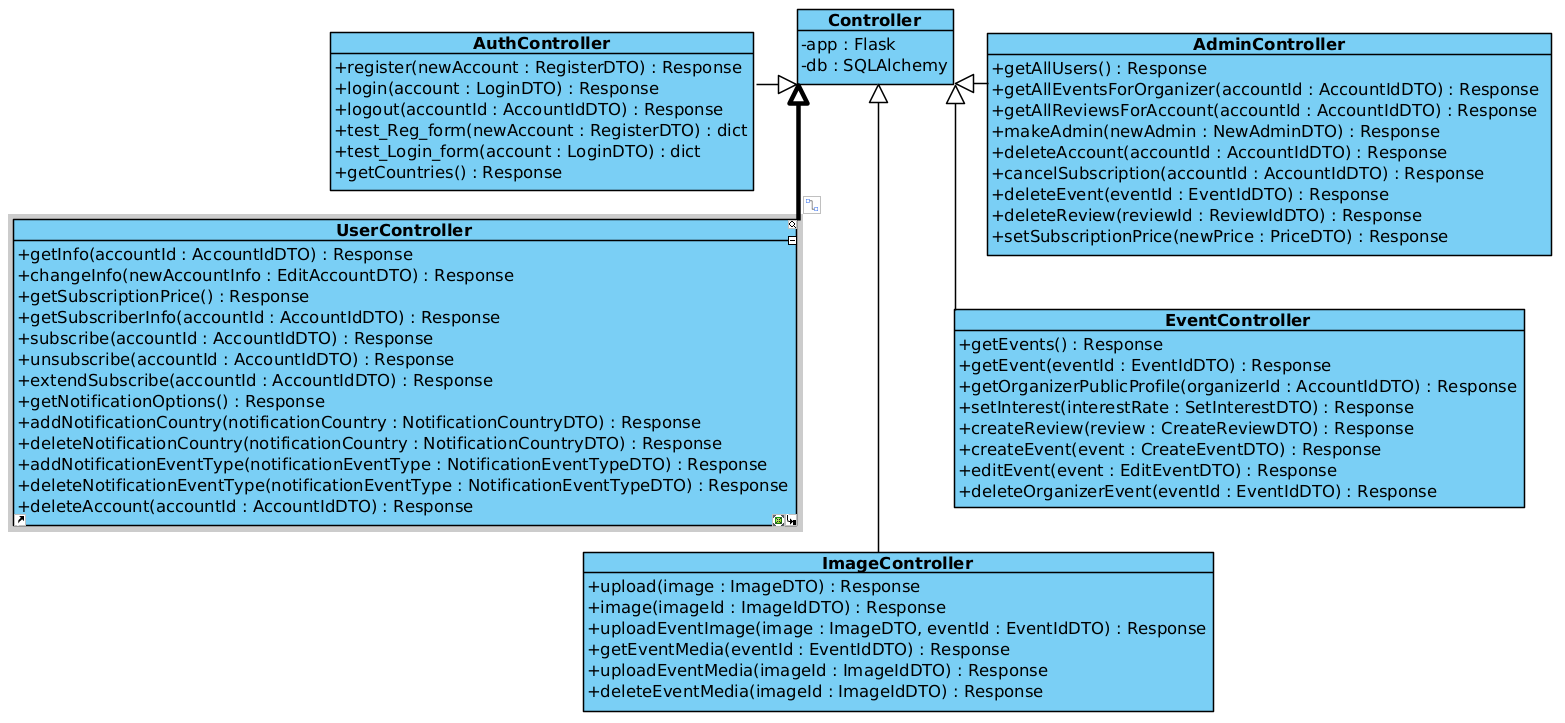
\includegraphics[width=1\textwidth]{dijagrami/dijagram_mvc_controllers.png}
				\caption{Dijagram klasa, dio Controllers}
			\label{fig:my_image}
			\end{figure}

			\pagebreak

			\begin{figure}[htbp]
				\centering
				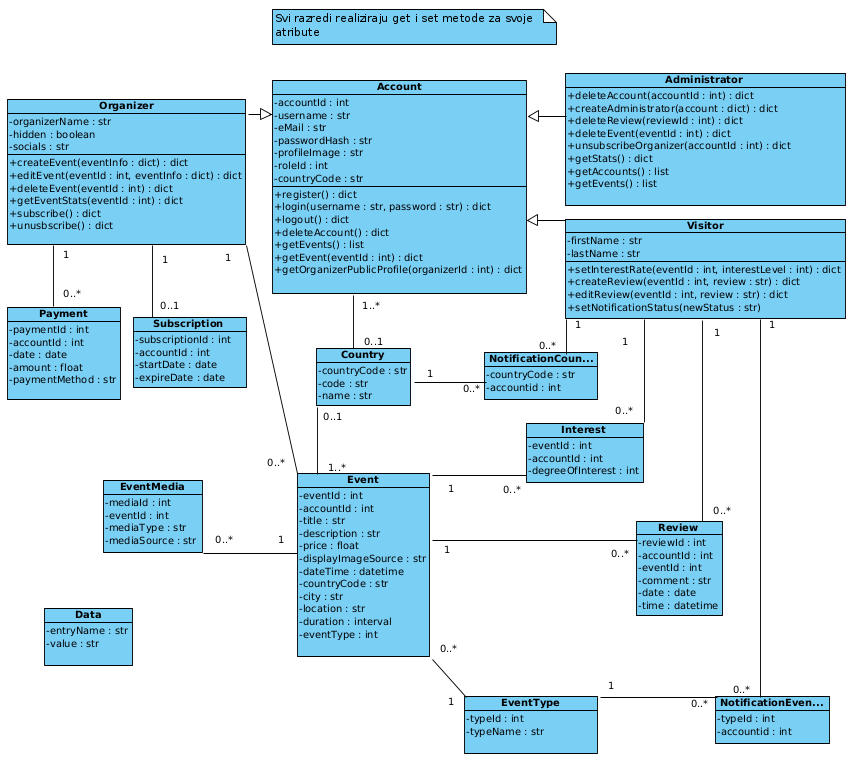
\includegraphics[width=1\textwidth]{dijagrami/dijagram_mvc_models.png}
				\caption{Dijagram klasa, dio Models}
			\label{fig:my_image}
			\end{figure}

			\pagebreak

			\eject
		
		\section{Dijagram stanja}
			
			
			\textbf{\textit{dio 2. revizije}}\\
			
			\textit{Potrebno je priložiti dijagram stanja i opisati ga. Dovoljan je jedan dijagram stanja koji prikazuje \textbf{značajan dio funkcionalnosti} sustava. Na primjer, stanja korisničkog sučelja i tijek korištenja neke ključne funkcionalnosti jesu značajan dio sustava, a registracija i prijava nisu. }
			
			
			\eject 
		
		\section{Dijagram aktivnosti}
			
			\textbf{\textit{dio 2. revizije}}\\
			
			 \textit{Potrebno je priložiti dijagram aktivnosti s pripadajućim opisom. Dijagram aktivnosti treba prikazivati značajan dio sustava.}
			
			\eject
		\section{Dijagram komponenti}
		
			\textbf{\textit{dio 2. revizije}}\\
		
			 \textit{Potrebno je priložiti dijagram komponenti s pripadajućim opisom. Dijagram komponenti treba prikazivati strukturu cijele aplikacije.}